\chapter{Erstellen eines Datensatzes}\label{chapter:dataset}
Ein wichtiger Bestandteil beim Entwickeln von künstlichen neuronalen Netzen ist
der unterliegende Datensatz, der zum Trainieren der Parameter der Netze
verwendet wird. Ein Machine-Learning-Modell ist nur so gut wie der verwendete
Datensatz. Dieser muss deshalb eine große Varianz der Daten repräsentieren. Das
bedeutet, dass ausreichend Einträge vorhanden sein müssen, um das Netzwerk auf
ähnliche, aber unbekannte Probleme vorzubereiten. Ein beliebter Datensatz ist
beispielsweise der MNIST-Datensatz \cite{6296535}, welcher unter anderem Bilder
von handgeschriebenen Ziffern bereitstellt. Anhand des MNIST-Beispiels bedeutet
eine große Varianz, dass eine Ziffer durch viele verschiedene Bilder
repräsentiert wird, die alle eine andere Perspektive des gleichen Kontexts
darstellen. Das Problem ist nämlich, dass eine handgeschriebene Ziffer immer anders aussieht. Um ein neuronales Netz also auf dieses Problem vorzubereiten, müssen verschiedenste Varianten zum Training bereitstehen.

In diesem Abschnitt soll nun ein Datensatz eingeführt werden, welcher keine
Daten für das Erkennen von Ziffern, aber für die die Bewegungserkennung
bereitstellt. Um diesen Datensatz zu erstellen, muss vorab geklärt werden, was
eine Bewegung eigentlich ist. Betrachtet man einen Punkt im Raum, dann
beschreibt eine Bewegung des Punktes die Änderung des Ortes eines Objekts über
die Zeit.  Bezogen auf den zu erstellenden Datensatz bedeutet dies, dass
einfache Bildaufnahmen von beweglichen (dynamischen) Objekten nicht ausreichen.
Um eine Bewegung aufzuzeichnen, müssen zeitlich aufeinander folgende Bilder, also Videos aufgenommen werden. Da der Datensatz später
dazu verwendet werden soll, ein neuronales Netz zu trainieren, welches
Bewegungen erkennt, müssen die zu erlernenden Bewegungen auch in diesem
Datensatz als Videos vertreten sein.

Bevor ein Modell für die Bewegungserkennung und -analyse trainiert wird, soll
zusätzlich untersucht werden, ob ein relativ kleiner Datensatz ausreichend ist,
um trotzdem gute Resultate beim Trainieren von neuronalen Netzen zu erzeugen. Da
diese Netze jedoch auf einen vielseitigen Datensatz zurückgreifen müssen, um
entsprechend gute Erkennungsraten zu erzeugen, ist die Idee, diesen kleinen
Datensatz künstlich zu erweitern. Interessant hierbei ist, ob ein künstlich
gedehnter Datensatz genau so gut geeignet ist, wie ein aufwändig erstellter
Datensatz bestehend aus realen Daten. Falls sich das Experiment als erfolgreich
herausstellt, liegt der Vorteil auf der Hand. Nämlich dass künstlich erzeugte
Datensätze wesentlich schneller auszuheben sind als Datensätze mit
ausschließlich realen Daten. Dies würde den Arbeitsaufwand für das Erstellen von
neuen komplexen Datensätzen um ein vielfaches verringern und gleichzeitig den
Fokus auf die eigentliche Forschungsarbeit verbessern.

Nun stellt sich natürlich die Frage, wie ein kleiner Datensatz künstlich
vergrößert werden kann. Künstlich bedeutet hier, dass das Vergrößern des
Datensatzes mithilfe von Algorithmen geschieht und vom Computer anstatt vom
Menschen durchgeführt wird. Die folgenden Beispiele richten sich nach
\cite{shorten2019}. Eine Möglichkeit ist es, die Daten zu augmentieren.  Dies
wird bereits häufig während des Trainings von neuronalen Netzen durchgeführt,
indem simple Transformationen wie Rotation, Translation und Verzerrung an den
Daten durchgeführt werden. Aber auch das Verändern des Gamma-Wertes eines Bildes
reicht in einigen Fällen aus, um eine Variation im Datensatz künstlich zu
erzeugen. Eine weitere Möglichkeit ist es, anderen neuronalen Netzen diese
Arbeit übernehmen zu lassen. Hierbei werden generative Modelle wie GANs
verwendet, um neue, bisher unbekannte Samples eines Datensatzes zu erzeugen.
Auch diese Idee ist nicht neu, jedoch beziehen sich die meisten Beispiele auf
das Generieren von einfachen Bildern. Da es sich bei dem zu erstellenden
Datensatz um Videos handelt, müssen die Techniken auf dieses Problem angewandt
werden. Neben den Inhalt von einzelnen Bildern muss das GAN als zusätzliche
Dimension also die Semantik zwischen einzelnen Frames bzw.  Bildern erlernen und
neu generieren können, da es keinen Sinn ergibt, dass der Kontext pro Videoframe
zufällig wechselt. Stattdessen wird gefordert, dass jeder erzeugte Frame von dem
vorherigen abhängt, sodass die Folge der Frames ein sinnvolles Video ergibt.

\section{GAN für Videos}
In diesem Abschnitt wird die Architektur von ViGAN vorgestellt und die Idee
dahinter erläutert. ViGAN steht für Video-Generative-Adversarial-Network und
wurde im Rahmen dieser Arbeit zum Erzeugen von neuen Videos aus einem
bestehendem Datensatz entwickelt. Gerade das Erstellen von Videos und das Labeln
der Bewegungen nimmt enorm viel Zeit in Anspruch. Mithilfe von ViGAN soll der
Aufwand reduziert werden. Hierbei wird untersucht, ob ein künstlich erweiterter
Datensatz für das Trainieren von neuronalen Netzen geeignet ist. In Kapitel
\ref{chapter:gans} werden verschiedene GANs und deren Probleme bzw. Vorteile
vorgestellt. Aufgrund der Vorteile von Wasserstein-GANs, nämlich die
Interpretationsmöglichkeit des Fehlers während des Trainings und die
Mode-Collapse-Resistenz, wird dieses als Grundarchitektur gewählt. Da häufig
GANs nur in Verbindung mit einzelnen Bildern verwendet werden, muss das WGAN
entsprechend angepasst werden, um Videos anstatt von Bildern zu erzeugen. Wie im
vorherigen Abschnitt besprochen, ist es wichtig, dass die Frames des Videos
zueinander passen und nicht aus dem Kontext gerissen werden. Wie in Abbildung
\ref{fig:vigan} dargestellt unterscheidet sich ViGAN nicht allzu sehr vom WGAN.
Der größte Unterschied besteht darin, dass 3D-Convolutional-Transpose- anstelle
der 2D-Convolutional-Transpose-Layer verwendet werden. Dies ermöglicht nicht nur
ein Hochskalieren des Bildes, sondern auch ein Erhöhen der Frameanzahl. Die Idee
dabei ist, dass das Netzwerk dadurch lernt, zusammenhängende Frames zu
generieren. Als Eingabe wird ein zufälliger Vektor $\vec{z}$ gewählt. Dann muss
das Netzwerk die eindimensionale Eingabe in eine vierdimensionale Struktur
umwandeln. Dies geschieht beim ViGAN mithilfe eines Fully-Connected-Layers mit
$5 \cdot 6 \cdot 8 \cdot 256$ Neuronen und einem Reshape-Layer, welcher die
Ausgabe des Fully-Connected-Layers in einen 4D-Tensor mit den Dimensionen $5
\times 6 \times 8 \times 256$ umstrukturiert. Die erste Dimension beschreibt
dabei immer die Anzahl der Frames, die zweite die Höhe, die dritte die Breite
und die vierte die Anzahl der Farbkanäle. Anschließend wird der Tensor mithilfe
eines Convolutional-Transpose-Layers vergrößert und die Frameanzahl erhöht. Der
Stride beträgt dabei 2, sodass eine Verdoppelung der Dimensionen stattfindet.
Insgesamt werden vier solcher Schichten hintereinander gereiht. Dabei entsteht
ein Ausgabevideo mit 80 Frames, wobei jeder Frame jeweils $96 \times 128 \times
3$ Pixelwerte besitzt.

\begin{figure}
    \centering
    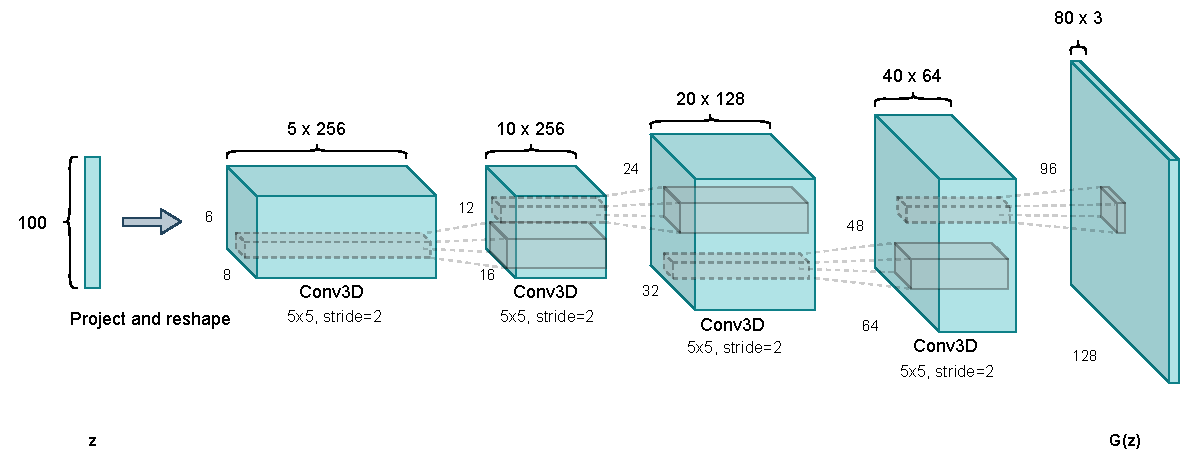
\includegraphics[width=\textwidth]{images/ViGAN.pdf}
    \caption{Architektur von ViGAN. Als Eingabe dient ein zufälliger Vektor $\vec{z}
    \in \mathbb{R}^{100}$. Dieser wird anschließend in fünf $6 \times 8 \times
    256$ Features umgewandelt. Um die relativ kleinen Frames in eine größere
    Auflösung zu skalieren, werden vier 3D-Convolutional-Transpose-Layer verwendet. Jedes
    dieser Schichten verwendet eine Kernelgröße von $5 \times 5 \times 5$ und
    einen Stride von 2.  Insgesamt ergibt sich also ein Stride von $2^4 = 16$,
    sodass die Eingabegröße von $5 \times 6 \times 8 \times 256$ auf 80x96x128x3
    hochskaliert wird.}
    \label{fig:vigan}
\end{figure}

\section{Training vom ViGAN}
Um ViGAN zu testen, werden einige Experimente durchgeführt, die untersuchen
sollen, ob die Ausgaben des GANs brauchbar sind. Unter anderem wird durch
Experimente herausgefunden, welcher Aufbau von Generator und Diskriminator (in
diesem Fall ist der Diskriminator ein Kritisierer) in einem stabilen Training
resultieren. Das Training wird auf eine GeForce RTX 3080 ausgelagert und dauert
im Schnitt 12 Stunden für 9000 Epochen bei einem Datensatz von 3 Videoclips mit
jeweils 840 Frames. Das größte Problem während des Trainings besteht darin, die
Trainingsdaten in den Speicher der Grafikkarte zu laden, da das Modell und die
Daten entsprechend groß sind. Daher kann nur mit einer Batch-Größe von 4
gearbeitet werden. Insgesamt wurden 8 Experimente durchgeführt, wobei sich die
Architekturen aus Tabelle \ref{table:stable-experiment} am stabilsten
herausstellten. Trotz des stabilen Trainings weisen die Ausgaben des
Generator-Netzwerkes einige Makel auf. Es entstehen zwar Videos, in denen eine
Bewegung stattfindet, jedoch sind auch Transitionen in der Inneneinrichtung
vorhanden. So verschwindet während des Videoclips beispielsweise eine Tür und es
erscheint eine Garnitur. Auf jeden Fall entstehen aber Räume, die so in der Art
nicht im Datensatz vorhanden sind. Leider wird auch nicht immer eine menschliche
Bewegung erzeugt, sodass sich zwar der Raum über die Zeit ändert, die Person
aber regungslos in diesem steht. Weitere Experimente haben gezeigt, dass auch
zwischen Personen interpoliert wird. Die sich bewegende Person verändert sich
also im Laufe der Zeit. Die Ergebnisse von ViGAN sind demnach zwar Videos,
dessen Frames voneinander abhängen, jedoch wurde es nicht geschafft, dynamische
Bewegungen mit konstanter Umgebung zu generieren.

\begin{table}
    \scriptsize
    \begin{tabularx}{\textwidth}{lXXXXll}
        \hline
        Input-Shape & Conv1 & Conv2 & Conv3 & Conv4 & Output-Shape & Parameter \\ \hline
        $5 \times 12 \times 16 \times 256$ & c=128 \newline s=2,2,2 & c=64 \newline s=2,2,2 & c=64 \newline s=2,2,2 & c=3 \newline s=1,2,2 & $40 \times 192 \times 256 \times 3$ & \num{3,07e7} \\ \hline

        $1 \times 3 \times 4 \times 96$ & c=96 \newline s=5,5,5 & c=48 \newline s=2,3,3 & c=16 \newline s=2,4,4 & c=3 \newline s=2,2,2 & $40 \times 360 \times 480 \times 3$ & \num{0,20e7} \\ \hline

        $1 \times 6 \times 8 \times 96$ & c=96 \newline s=5,5,5 & c=48 \newline s=3,3,3 & - & c=3 \newline s=4,4,4 & $40 \times 360 \times 480 \times 3$ & \num{0,22e7} \\ \hline

        $10 \times 20 \times 45 \times 256$ & c=128 \newline s=1,1,1 & c=64 \newline s=2,2,2 & - & c=3 \newline s=2,2,2 & $40 \times 80 \times 180 \times 3$ & \num{2,40e8} \\ \hline

        $5 \times 3 \times 4 \times 256$ & c=256 \newline s=1,1,1 & c=128 \newline s=2,2,2 & c=128 \newline s=2,2,2 & c=3 \newline s=3,3,3 & $60 \times 36 \times 48 \times 3$ & \num{1,60e7} \\ \hline

        $5 \times 3 \times 4 \times 512$ & c=256 \newline s=2,2,2 & c=128 \newline s=2,2,2 & - & c=3 \newline s=3,3,3 & $60 \times 36 \times 48 \times 3$ & \num{2,37e7} \\ \hline

        $5 \times 6 \times 8 \times 256$ & c=128 \newline s=2,2,2 & c=64 \newline s=2,2,2 & c=32 \newline s=2,2,2 & c=3 \newline s=2,2,2 & $80 \times 96 \times 128 \times 3$ & \num{1,17e7} \\ \hline

        $15 \times 12 \times 16 \times 256$ & c=128 \newline s=2,2,2 & c=64 \newline s=2,2,2 & - & c=3 \newline s=2,2,2 & $120 \times 96 \times 128 \times 3$ & \num{8,03e7} \\ \hline
    \end{tabularx}
    \caption{Stabile Konfigurationen für ViGAN. Es wurde untersucht, welche Konfigurationen
    zu einem stabilen Training führen. Außerdem wurde versucht, die Anzahl der
    erzeugten Frames so hoch wie möglich zu halten. Die Convolutional-Layer
    besitzen alle $5 \times 5 \times 5$ Kernels. Die Parameter $c$ und $s$ beschreiben entsprechend die Channels und Strides der Convolutional-Layer.}
    \label{table:stable-experiment}
\end{table}

\section{GAN für Schlüsselpunktanimationen}
Da das ViGAN einige Probleme aufgewiesen hat, wurde eine alternative Methode
entwickelt, um Bewegungen effizienter und genauer zu generieren. Weil sich diese
Arbeit mit der Bewegungserkennung auseinandersetzt und ViGAN zu viel
bewegungsunabhängige Transitionen in den Videos erzeugt, soll eine neue Methode
vorgestellt werden, die direkt Bewegungsinformationen künstlich erzeugen kann.
Auch in dieser Methode wird ein GAN verwendet, nur diesmal wird die Information
einer Bewegung wesentlich genauer betrachtet. Das Ziel ist ein schnelleres
Training des Netzwerks sowie ein geringerer Speicherverbrauch. Ein großer
Nachteil beim ViGAN ist, dass viele unnötige Informationen mit generiert werden.
Für die eigentliche Bewegungserkennung ist eine Veränderung des Raumes über die
Zeit eher uninteressant. Nur die Bewegung selbst interessiert dabei.
Die Idee ist nun, dass anstatt Videos mit sich bewegenden Menschen in Räumen erzeugt werden, nun Animationen
bestehend aus Schlüsselpunkten des menschlichen Körpers generiert werden. Die
Folge dieser Schlüsselpunkte soll schließlich eine Bewegung darstellen.
Extrahiert man die Schlüsselpunkte aus entsprechenden Videos, die eine
Bewegungsart beinhalten, so wird der eigentliche Datensatz um ein vielfaches
reduziert, jedoch bleibt die zu betrachtende Information gleich. Genau
wie beim ViGAN wird hier ebenfalls ein WGAN als Grundarchitektur verwendet. Im
Grunde verhält sich das Netzwerk ähnlich, außer dass es einzelne
Bilder anstatt Videos generiert. Genauer gesagt, wird ein
Conditional-Wasserstein-GAN verwendet, sodass das jeweilige Label mit als
Eingabe fungieren kann, um den Generator zu zwingen, eine Ausgabe einer
bestimmten Klasse zu erzeugen. Dadurch kann gesteuert werden, welche Art von
Ausgabe dieser Generator liefert, was unabdingbar für das Erzeugen eines
kompletten Datensatzes ist. Andernfalls erhält man zwar künstlich erzeugte
Bewegungen, jedoch ist die Klasse bzw. das Label unbekannt. Demnach wär die
einzige Alternative das Trainieren von $n$ WGANs, wobei $n$ die Anzahl der im
System vorkommenden Klassen beschreibt, also ein WGAN pro Klasse. Da dies eine
sehr unelegante Lösung wär, wird versucht ein cWGAN entsprechend Abschnitt
\ref{section:cwgan-gp} zu implementieren, welches Proben aus $n$ verschiedenen
Klassen erzeugen kann. Mithilfe eines Labels als Eingabe soll gesteuert werden
können, zu welcher Klasse das Erzeugnis gehören soll

Eine Bewegung bestehend aus $N$ Frames und $k$ Schlüsselpunkten, die jeweils
eine Position im zweidimensionalen Raum und eine Auftrittswahrscheinlichkeit
besitzen, können mithilfe eines Bildes repräsentiert werden. Ein solches Bild
besitzt damit eine Größe von $N \times k \times 3$. Da später Modelle
verwendet werden sollen, welche auf dem \textit{COCO Keypoints Dataset}
\cite{lin2015microsoft} trainiert wurden und somit 17 Schlüsselpunkte von
Menschen in Bildern erkennen, wird $k = 17$ gewählt. Zudem wird die Anzahl der
Frames auf $N = 60$ gesetzt. Es wird hier also angenommen, dass entsprechende
Bewegungen innerhalb von 60 Frames eindeutig erkennbar sind. Die Ausgaben des
GANs sind dementsprechend im Format $60 \times 17 \times 3$. In Abbildung
\ref{fig:motion-images} werden beispielhaft drei Bewegungsarten zu Bilder
kodiert und deren ersten 10 Frames dargestellt, die durch die ersten 10 Reihen
des jeweiligen Bildes repräsentiert werden. Auf Basis dieser Bilder wird nun ein
GAN entwickelt, welches neue Bewegungen des gleichen Typs erzeugen soll. Mit
anderen Worten, das GAN soll lernen, ähnliche Bilder zu erzeugen, die wiederum
in Schlüsselpunktframes dekodiert werden können. Wenn dieses Experiment
erfolgreich ist, dann kann der Generator als Datensatzerzeuger für die
Bewegungserkennung verwendet werden.

\begin{figure}
    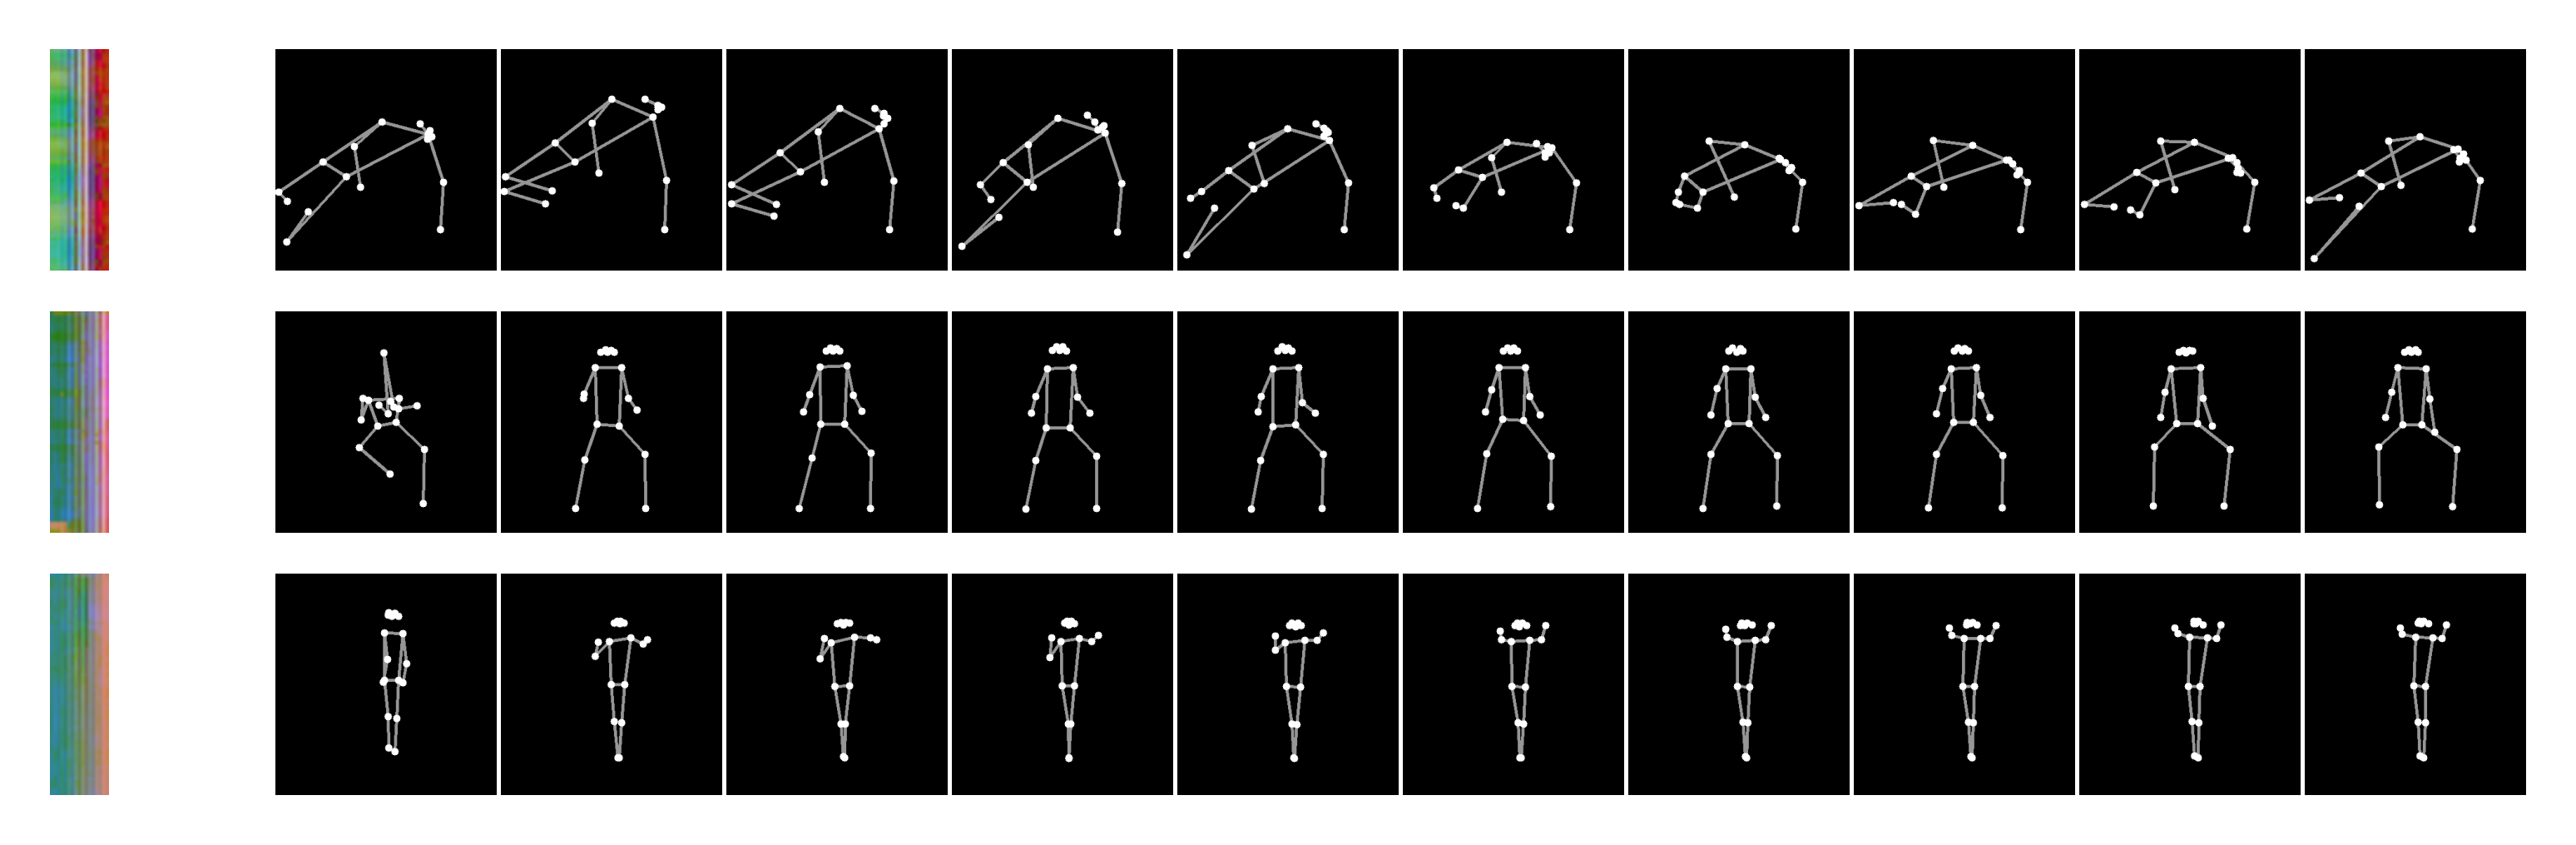
\includegraphics[width=\textwidth]{images/motion_image.png}
    \caption{Die Frames von Schlüsselpunktanimationen können als
    zweidimensionale Bilder repräsentiert werden. Die erste Reihe stellt eine
    Liegestütz-, die zweite eine Bankpress- und die dritte eine Hantelbewegung
    dar. Die erste Spalte zeigt jeweils das kodierte Bild, während die
    restlichen Spalten die ersten 10 Frames der Bewegung zeigen.}
    \label{fig:motion-images}
\end{figure}

\section{Training vom KpGAN}
Für das Training wurde der UCF-101-Datensatz \cite{ucf101} verwendet. Dieser
enthält sportliche Aktivitäten in Form von Videos, sodass diese vorerst in
Schlüsselpunktanimationen umgewandelt werden müssen. Anstatt jeden Frames jedes
Videos per Hand zu bearbeiten und Schlüsselpunkte zu annotieren, wird dies
mithilfe von MoveNet \cite{movenet} automatisiert erledigt. Die Schlüsselpunkte
der jeweiligen Frames werden in Bilder wie in Abbildung \ref{fig:motion-images}
kodiert und als Eingabe in das KpGAN gegeben. Die Experimente verlaufen ähnlich
wie beim ViGAN, es werden jedoch andere Parameter gewählt, die pro Experiment
verändert werden. Im ersten Schritt wurde untersucht, welche Netzkonfiguration
stabil beim Training ist. Der finale Aufbau ist in Abbildung \ref{fig:kpgan} zu
sehen und wurde wie beim ViGAN durch unterschiedliche Versuche herausgefunden.
Anschließend wurde untersucht, wie sich das Verhalten während des Trainings
ändert, wenn wahlweise Batch-Normalisierung- und Bias-Schichten hinzugefügt
werden.  Außerdem wurde geschaut, welche Aktivierungsfunktion in der letzten
Schicht zu den besten Ergebnissen führt. Dafür wurden Aktivierungen durch
Sigmoid- und Tangens-Hyperbolicus-Funktionen realisiert. Konfigurationen mit
Bias-Layer, aber ohne Batch-Normalisierung führten zu den besten Ergebnissen.
Abbildung \ref{fig:kpgan-example} zeigt eine zufällige Liegestützbewegung, die
vom KpGAN erzeugt wurde. Für das Training stand eine GeForce RTX 3080 zur
Verfügung und 3000 Epochen dauerten $< 1$ Minuten. Grundsätzlich sind die
Ergebnisse zufriedenstellend, sodass dieses GAN verwendet werden kann, um
verschiedene Bewegungen zu erzeugen.

\begin{figure}
    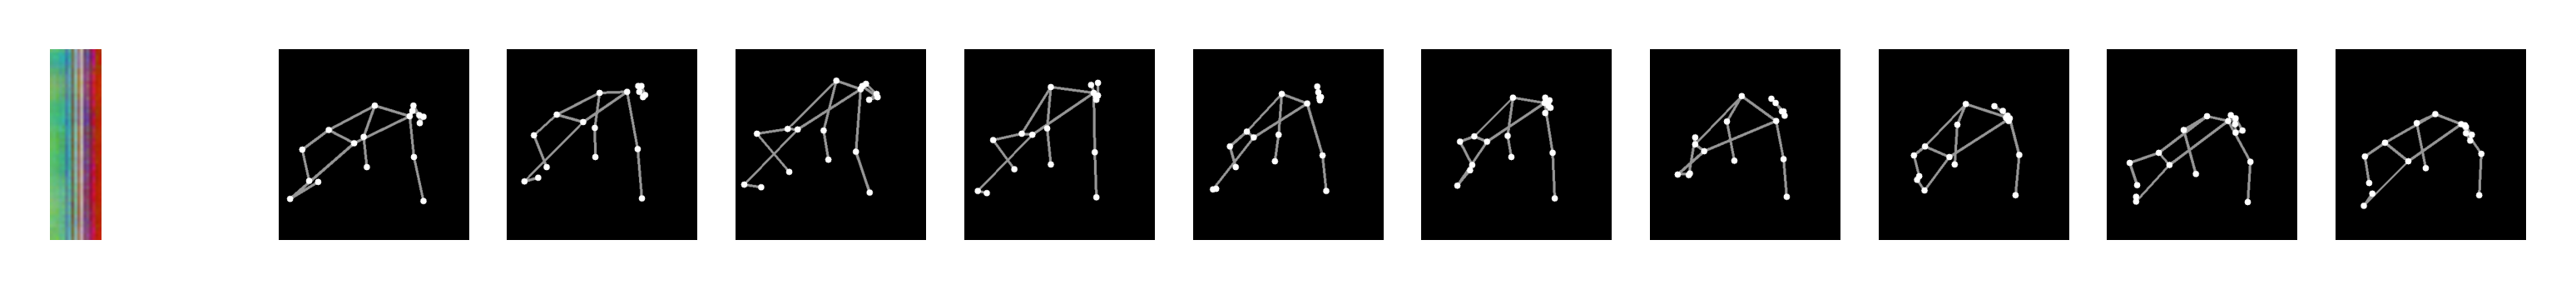
\includegraphics[width=\textwidth]{images/kpgan-example.png}
    \caption{Beispielausgabe vom KpGAN. Links ist die direkte Ausgabe des
    Netzwerks. Von links nach rechts werden chronologisch die ersten 10
    dekodierten Frames dargestellt.}
    \label{fig:kpgan-example}
\end{figure}

\begin{figure}
    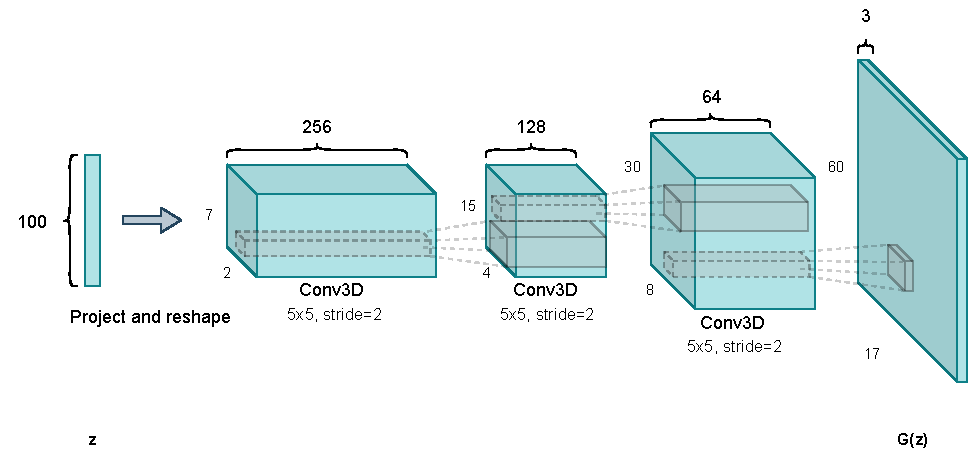
\includegraphics[width=\textwidth]{images/KpGAN.pdf}
    \caption{Architektur von KpGAN zum Generieren von 60 Frames einer
    Schlüs\-sel\-punkt\-anima\-tion. Die Eingabe ist ein Vektor, welcher
  zunächst in das Format $7 \times 2 \times 256$ gebracht wird und das Label
der zu erzeugenden Bewegungsart. Anschließend wird mithilfe von insgesamt vier
Convolutional-Transpose-Layer eine Ausgabe im Format $60 \times 17 \times 3$
erzeugt. Es werden entsprechend 256, 128, 64 und 3 Filter für die Schichten
verwendet.}
    \label{fig:kpgan}
\end{figure}
